\section{A drón kontroller modellje MATLAB Simulinkben}
A drón vezérlőrendszerének modellezését és szimulációját MATLAB Simulink környezetben végeztem el, az UAV Toolbox segítségével. Ez az eszközkészlet kifejezetten hasznos a drónok és más légi járművek fejlesztése során, mivel előre elkészített modulokat és sablonokat kínál a vezérlési, navigációs és repülésdinamikai modellezéshez.

\begin{figure}[H]
	\centering
	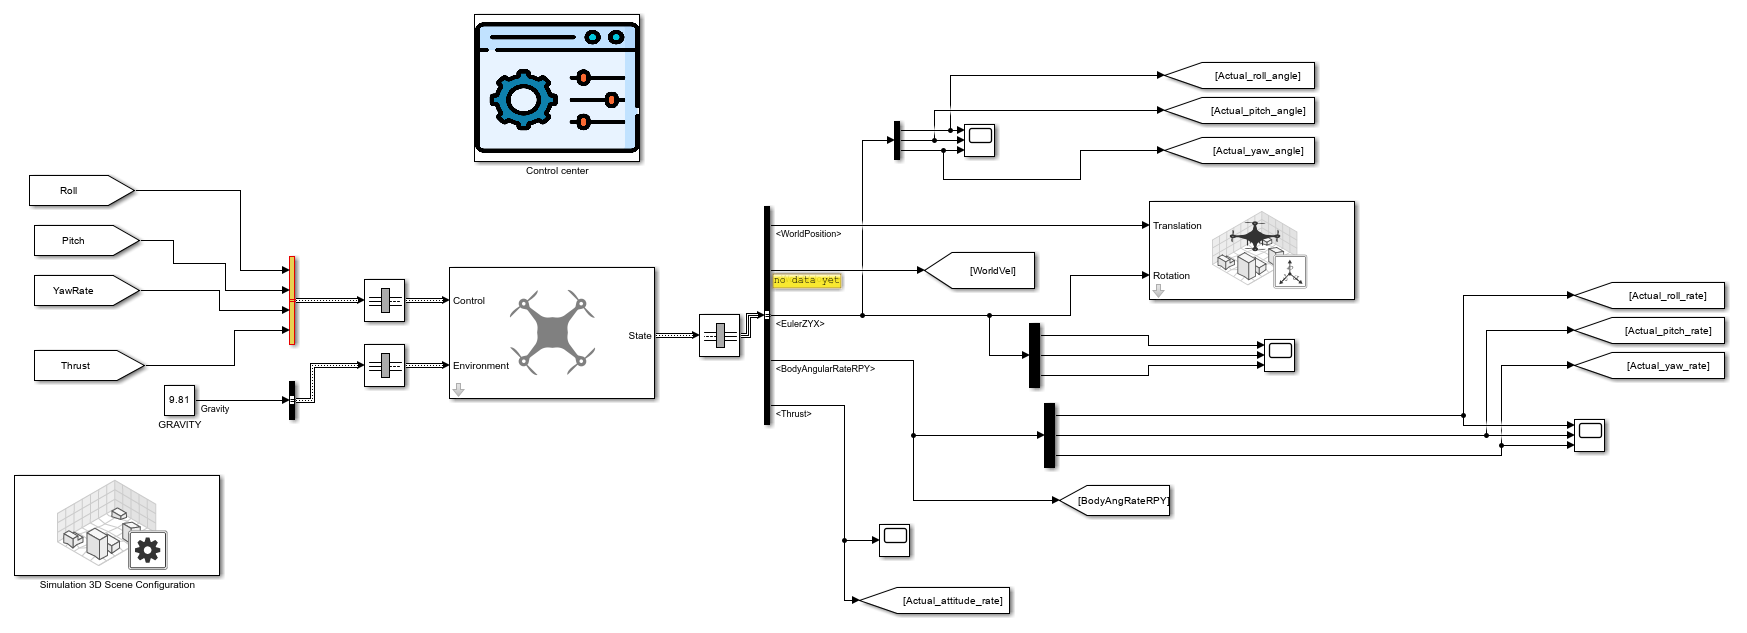
\includegraphics[scale=0.3]{control-arch.png}
	\caption{Drón kontroller architechtúrája}
	\label{Drón kontroller architechtúrája SIMULINK környezetben}
\end{figure}

\begin{figure}[H]
	\centering
	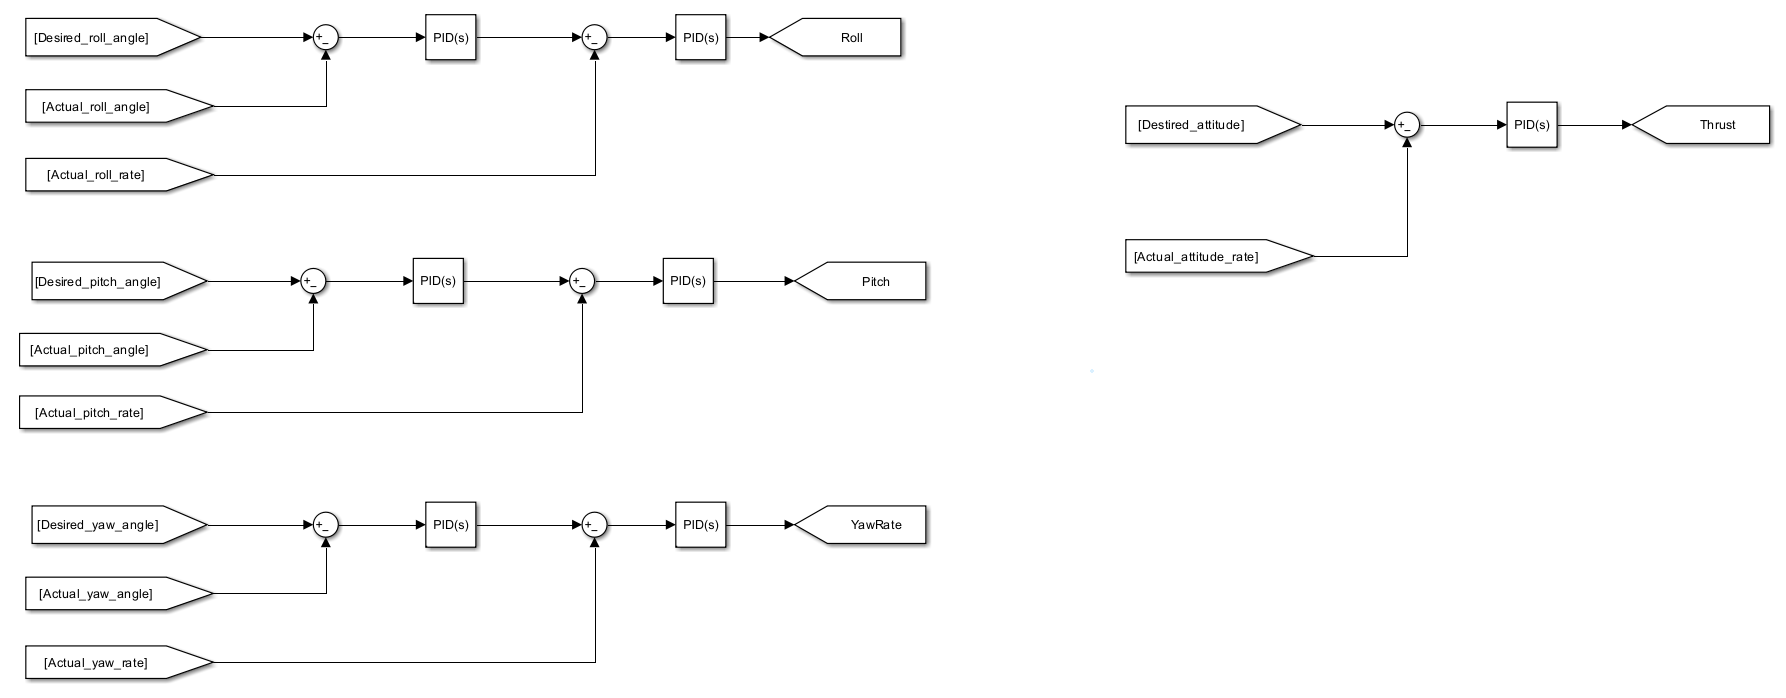
\includegraphics[scale=0.3]{cascade-pid-control.png}
	\caption{Drón visszacsatolt rendszerének cascade szabályzása}
	\label{Drón visszacsatolt rendszerének cascade szabályzása}
\end{figure}
